



\documentclass[nohyperref]{article}

\usepackage{algpseudocode}
\renewcommand{\algorithmicrequire}{\textbf{Input:}}  
\renewcommand{\algorithmicensure}{\textbf{Output:}} 
\usepackage{microtype}
\usepackage{graphicx}
\usepackage{subfigure}
\usepackage{booktabs} \newcommand{\fix}[1]{\textcolor{black}{#1}}
\usepackage{pgfplots}
\usetikzlibrary{pgfplots.groupplots}
\pgfplotsset{compat=1.3}
\usepackage{tikz}
\usetikzlibrary{patterns}
\usepackage{pgf-pie}
\usepackage{pifont} 
\newcommand{\okmark}{{\textbf{\textcolor[rgb]{0.1, 0.5, 0.1}{$\checkmark$}}}}
\newcommand{\ngmark}{{\textbf{\color{red}{\ding{55}}}}}

\definecolor{battleshipgrey}{rgb}{0.3, 0.3, 0.3}
\definecolor{brilliantrose}{rgb}{1.0, 0.33, 0.64}
\definecolor{americanrose}{rgb}{1.0, 0.01, 0.24}
\definecolor{jweigreen}{rgb}{0,0.45,0.24}
\definecolor{bluegray}{rgb}{0.1, 0.1, 0.4}
\definecolor{ao(english)}{rgb}{0.0, 0.5, 0.0}
\definecolor{blanchedalmond}{rgb}{1.0, 0.92, 0.8}
\definecolor{atomictangerine}{rgb}{1.0, 0.6, 0.4}
\definecolor{chocolate(web)}{rgb}{0.82, 0.41, 0.12}
\definecolor{bananayellow}{rgb}{1.0, 0.88, 0.21}
\definecolor{goldenbrown}{rgb}{0.6, 0.4, 0.08}
\definecolor{aliceblue}{rgb}{0.94, 0.97, 1.0}
\definecolor{beige}{rgb}{0.96, 0.96, 0.86}
\definecolor{babyblue}{rgb}{0.54, 0.81, 0.94}
\definecolor{camel}{rgb}{0.76, 0.6, 0.42}
\definecolor{cinnamon}{rgb}{0.82, 0.41, 0.12}
\newcommand{\battleshipgrey}[1]{{\color{battleshipgrey}{#1}}}
\newcommand{\americanrose}[1]{{\color{americanrose}{#1}}}
\newcommand{\jweigreen}[1]{{\color{jweigreen}{#1}}}
\newcommand{\darkgreen}[1]{{\color{ao(english)}{#1}}}
\newcommand{\aliceblue}[1]{{\color{aliceblue}{#1}}}
\newcommand{\beige}[1]{{\color{beige}{#1}}}
\newcommand{\babyblue}[1]{{\color{babyblue}{#1}}}
\newcommand{\camel}[1]{{\color{camel}{#1}}}
\newcommand{\cinnamon}[1]{{\color{cinnamon}{#1}}}
\newcommand\tikzmark[2]{\tikz[remember picture,baseline] \node[above, outer sep=0pt, inner sep=0pt] (#1){\phantom{#2}};} 
\usepackage{hyperref}


\newcommand{\theHalgorithm}{\arabic{algorithm}}




\usepackage[accepted]{icml2023}

\usepackage{amsmath}
\usepackage{amssymb}
\usepackage{mathtools}
\usepackage{amsthm}
\usepackage{multirow}
\usepackage{pgfplots}
\usepackage[capitalize,noabbrev]{cleveref}
\theoremstyle{plain}
\newtheorem{theorem}{Theorem}[section]
\newtheorem{proposition}[theorem]{Proposition}
\newtheorem{lemma}[theorem]{Lemma}
\newtheorem{corollary}[theorem]{Corollary}
\theoremstyle{definition}
\newtheorem{definition}[theorem]{Definition}
\newtheorem{assumption}[theorem]{Assumption}
\theoremstyle{remark}
\newtheorem{remark}[theorem]{Remark}

\usepackage[textsize=tiny]{todonotes}


\icmltitlerunning{Multimodal Chain-of-Thought Reasoning in Language Models}

\begin{document}

\twocolumn[
\icmltitle{Multimodal Chain-of-Thought Reasoning in Language Models}





\icmlsetsymbol{equal}{*}
\begin{icmlauthorlist}
\icmlauthor{Zhuosheng Zhang}{s}
\icmlauthor{Aston Zhang}{a}
\icmlauthor{Mu Li}{a}
\icmlauthor{Hai Zhao}{s}
\icmlauthor{George Karypis}{a}
\icmlauthor{Alex Smola}{a}
\end{icmlauthorlist}

\icmlaffiliation{s}{Shanghai Jiao Tong University}
\icmlaffiliation{a}{Amazon Web Services}

\icmlcorrespondingauthor{Zhuosheng Zhang (work done at Amazon Web Services)}{zhangzs@sjtu.edu.cn}
\icmlcorrespondingauthor{Aston Zhang}{az@astonzhang.com}

\icmlkeywords{Machine Learning, ICML}

\vskip 0.3in
]





\printAffiliationsAndNotice{}  

\begin{abstract}
Large language models (LLMs) have shown impressive performance on complex reasoning by leveraging chain-of-thought (CoT) prompting to generate intermediate reasoning chains as the rationale to infer the answer. However, existing CoT studies have focused on the language modality. {We propose Multimodal-CoT that incorporates language (text) and vision (images) modalities into a two-stage framework that separates rationale generation and answer inference. 
In this way, answer inference can leverage better generated rationales that are based on multimodal information.}
With Multimodal-CoT, our model under 1 billion parameters outperforms the previous state-of-the-art LLM (GPT-3.5) by 16 percentage points (75.17\%$\rightarrow$91.68\% accuracy) and even surpasses human performance on the ScienceQA benchmark. 
Code is publicly available.\footnote{\url{https://github.com/amazon-science/mm-cot}}





\end{abstract}

\vspace{-3.8mm}
\section{Introduction}
\label{intro}
Imagine reading a textbook with no figures or tables. Our ability to knowledge acquisition is greatly strengthened by jointly modeling diverse data modalities, such as vision, language, and audio. Recently, large language models (LLMs) \citep{brown2020language, lamda, gopher, palm} have shown impressive performance in complex reasoning by generating intermediate reasoning steps before inferring the answer. The intriguing technique is called chain-of-thought (CoT) reasoning \citep{cot_wei,kojima2022large,zhang2022automatic}. 





However, existing studies related to CoT reasoning are largely isolated in the language modality \citep{wang2022rationale,zhou2022least,lu2022dynamic,fu2022complexity}, with little consideration of multimodal scenarios. To elicit CoT reasoning in multimodality, we advocate a Multimodal-CoT paradigm. Given the inputs in different modalities, Multimodal-CoT decomposes multi-step problems into intermediate reasoning steps (rationale) and then infers the answer. Since vision and language are the most popular modalities, we focus on those two modalities in this work. An example is shown in Figure \ref{fig_examples}. In general, there are two ways to elicit Multimodal-CoT reasoning as follows: (i) prompting LLMs and (ii) fine-tuning small models.\footnote{In this work, we refer to small models as models with less than 1 billion parameters (hereinafter dubbed as 1B-models).}

\begin{figure}[t]
  \begin{center}
   \includegraphics[width=1\columnwidth]{figures/fig-example.pdf}
  \end{center}
  \vspace{-3.6mm}
  \caption{Example of the multimodal CoT task.}
    \vspace{-7mm}
  \label{fig_examples}
\end{figure}


The most immediate way to perform Multimodal-CoT is to transform the input of different modalities into one modality and prompt LLMs to perform CoT. {For example}, it is possible to extract the caption of an image by a captioning model and then concatenate the caption with the original language input to be fed into LLMs \citep{lu2022learn}. However, {there is severe information loss in the captioning process; thus, using the captions (as opposed to vision features) may suffer from a lack of mutual synergy in the representation space of different modalities.}

\begin{table*}[htb]
\centering
\vspace{-3mm}
\renewcommand\tabcolsep{4.2pt} \small
\caption{Typical CoT techniques (FT: fine-tuning; KD: knowledge distillation). Segment 1: in-context learning techniques; Segment 2: fine-tuning techniques. To the best of our knowledge, our work is the first to study CoT reasoning in different modalities. Besides, we focus on 1B-models, without relying on the outputs of LLMs. \label{tab:cot_methods}
}
\begin{tabular}{lcccccc} 
\toprule
\textbf{Models} & \textbf{Mutimodal} & \textbf{w/o LLM}  & \textbf{Model / Engine}  & \textbf{Training}  & \textbf{CoT Role} & \textbf{CoT Source} \\ 
\midrule
Zero-Shot-CoT~\citep{kojima2022large} & \ngmark & \ngmark & GPT-3.5 (175B)  & ICL  & Reasoning & Template  \\
Few-Shot-CoT~\citep{cot_wei} & \ngmark & \ngmark   & PaLM (540B) & ICL & Reasoning & Hand-crafted \\
Self-Consistency-CoT~\citep{cot_wei_sc} & \ngmark & \ngmark & Codex  (175B) & ICL  & Reasoning& Hand-crafted   \\
Least-to-Most Prompting~\citep{zhou2022least}& \ngmark& \ngmark  & Codex (175B)  & ICL & Reasoning & Hand-crafted   \\
Retrieval-CoT~\citep{zhang2022automatic} & \ngmark& \ngmark  & GPT-3.5 (175B) & ICL  & Reasoning & Auto-generated  \\
PromptPG-CoT~\citep{lu2022dynamic} & \ngmark & \ngmark & GPT-3.5 (175B) & ICL & Reasoning  & Hand-crafted   \\
Auto-CoT~\citep{zhang2022automatic} & \ngmark & \ngmark  & Codex (175B)  & ICL & Reasoning  & Auto-generated \\
Complexity-CoT~\citep{fu2022complexity}& \ngmark & \ngmark  & GPT-3.5 (175B) & ICL  & Reasoning & Hand-crafted  \\
Few-Shot-PoT~\citep{chen2022program} & \ngmark & \ngmark & GPT-3.5 (175B) & ICL & Reasoning  & Hand-crafted  \\ 
\midrule
UnifiedQA~\citep{lu2022learn}& \ngmark  & \okmark   & T5 (770M)& FT & Explanation  & Crawled\\
Fine-Tuned T5 XXL~\citep{magister2022teaching}  & \ngmark & \ngmark  & T5 (11B)& KD & Reasoning  & LLM-generated \\
Fine-Tune-CoT \citep{ho2022large} & \ngmark & \ngmark  & GPT-3 (6.7B) & KD & Reasoning  & LLM-generated \\
Multimodal-CoT (our work) & \okmark &\okmark  & T5 (770M)& FT & Reasoning  & Crawled   \\ 
\bottomrule
\end{tabular}
\vspace{-5mm}
\end{table*}


{To facilitate the interaction between modalities, another potential solution is to fine-tune smaller language models (LMs) by fusing multimodal features \citep{zhang2023universal}. As this approach allows the flexibility of adjusting model architectures to incorporate multimodal features, we study fine-tuning models in this work instead of prompting LLMs. The key challenge is that language models under 100 billion parameters tend to generate hallucinated rationales that mislead the answer inference \citep{ho2022large,magister2022teaching,ji2022survey}.}



{To mitigate the challenge of hallucination, we propose Multimodal-CoT that incorporates language (text) and vision (images) modalities into a two-stage framework that separates rationale generation and answer inference. 
In this way, answer inference can leverage better generated rationales that are based on multimodal information.} 
Our experiments are conducted on the ScienceQA benchmark \citep{lu2022learn}, which is the latest multimodal reasoning benchmark with annotated reasoning chains. Experimental results show that our method surpasses the previous state-of-the-art GPT-3.5 model by +16\% (75.17\%$\rightarrow$91.68\%) on the benchmark. Our contributions are summarized as follows:


(i) {To the best of our knowledge, this work is the first to study CoT reasoning in different modalities.}

(ii) We propose a two-stage framework by fine-tuning language models to fuse vision and language representations to perform Multimodal-CoT. The model is able to generate informative rationales to facilitate inferring final answers.

(iii) Our method achieves new state-of-the-art performance on the ScienceQA benchmark, outperforming accuracy of GPT-3.5 by 16\% and even surpassing human performance.





















\section{Background}  

This section reviews recent progress of eliciting CoT reasoning by prompting and fine-tuning language models.

\subsection{CoT Reasoning with LLMs}
Recently, CoT has been widely used to elicit the multi-step reasoning abilities of LLMs \citep{cot_wei}. Concretely, CoT techniques encourage the LLM to generate intermediate reasoning chains for solving a problem. Studies have shown that LLMs can perform CoT reasoning with two major paradigms of techniques: Zero-Shot-CoT \citep{kojima2022large} and Few-Shot-CoT \citep{cot_wei,zhang2022automatic}. For Zero-Shot-CoT, \citet{kojima2022large} showed that LLMs are decent zero-shot reasoners by adding a prompt like ``Let’s think step by step" after the test question to invoke CoT reasoning. For Few-Shot-CoT, a few step-by-step reasoning demonstrations are used as conditions for inference. Each demonstration has a question and a reasoning chain that leads to the final answer. The demonstrations are commonly obtained by hand-crafting or automatic generation. The corresponding techniques are thus referred to as Manual-CoT \citep{cot_wei} and Auto-CoT \citep{zhang2022automatic}. 

With effective demonstrations, Few-Shot-CoT often achieves stronger performance than Zero-Shot-CoT and has attracted more research interest. Therefore, most recent studies focused on how to improve Few-Shot-CoT. Those studies are categorized into two major research lines: (i) optimizing the demonstrations; (ii) optimizing the reasoning chains. Table \ref{tab:cot_methods} compares typical CoT techniques.

\paragraph{Optimizing Demonstrations} The performance of Few-Shot-CoT relies on the quality of demonstrations. As reported in \citet{cot_wei}, using demonstrations written by different annotators results in dramatic accuracy disparity in a symbolic reasoning task. Beyond hand-crafting the demonstrations, recent studies have investigated ways to optimize the demonstration selection process. Notably, \citet{rubin2021learning} retrieved the semantically similar demonstrations with the test instance. However, this approach shows a degraded performance when there are mistakes in the reasoning chains \citep{zhang2022automatic}. To address the limitation, \citet{zhang2022automatic} found that the key is the diversity of demonstration questions and proposed Auto-CoT: (i) partition questions of a given dataset into a few clusters; (ii) sample a representative question from each cluster and generate its reasoning chain using Zero-Shot-CoT with simple heuristics. In addition, reinforcement learning (RL) and complexity-based selection strategies were also proposed to obtain effective demonstrations. \citet{fu2022complexity} chose examples with complex reasoning chains (i.e., with more reasoning steps) as the demonstrations. \citet{lu2022dynamic} trained an agent to find optimal in-context examples from a candidate pool and maximize the prediction rewards on given training examples when interacting with GPT-3.5.


\paragraph{Optimizing Reasoning Chains} A notable way to optimize reasoning chains is problem decomposition.  \citet{zhou2022least} proposed least-to-most prompting to decompose complex problems into sub-problems and then solve these sub-problems sequentially. As a result, solving a given sub-problem is facilitated by the answers to previously solved sub-problems. Similarly, \citet{khot2022decomposed} used diverse decomposition structures and designed different prompts to answer each sub-question. In addition to prompting the reasoning chains as natural language texts, \citet{chen2022program} proposed program-of-thoughts (PoT), which modeled the reasoning process as a program and prompted LLMs to derive the answer by executing the generated programs. Another trend is to vote over multiple reasoning paths for a test question. \citet{cot_wei_sc} introduced a self-consistency decoding strategy to sample multiple outputs of LLMs and then took a majority over the final answers. \citet{wang2022rationale} and \citet{li2022advance} introduced randomness in the input space to produce more diverse outputs for voting.

\subsection{Eliciting CoT Reasoning by Fine-Tuning Models}
A recent interest is eliciting CoT reasoning by fine-tuning language models. \citet{lu2022learn} fine-tuned the encoder-decoder T5 model on a large-scale dataset with CoT annotations. However, a dramatic performance decline is observed when using CoT to infer the answer, i.e., generating the reasoning chain before the answer (reasoning). Instead, CoT is only used as an explanation after the answer. \citet{magister2022teaching} and \citet{ho2022large} employed knowledge distillation by fine-tuning a student model on the chain-of-thought outputs generated by a larger teacher model. The proposed methods showed performance gains in arithmetic, commonsense, and symbolic reasoning tasks. 

{There is a key challenge in training 1B-models to be CoT reasoners.} As observed by \citet{cot_wei}, models under 100 billion parameters tend to produce illogical CoT that leads to wrong answers. In other words, it might be harder for 1B-models to generate effective CoT than directly generating the answer. It becomes even more challenging in a multimodal setting where answering the question also requires understanding the multimodal inputs. In the following part, we will explore the challenge of Multimodal-CoT and investigate how to perform effective multi-step reasoning.


\section{Challenge of Multimodal-CoT}\label{sec:prelim}
Existing studies have suggested that the CoT reasoning ability may emerge in language models at a certain scale, e.g., over 100 billion parameters \citep{wei2022emergent}. However, it remains an unresolved challenge to elicit such reasoning abilities in 1B-models, let alone in the multimodal scenario. {This work focuses on 1B-models as they can be fine-tuned and deployed with consumer-grade GPUs (e.g., 32G memory).}
In this section, we will investigate why 1B-models fail at CoT reasoning and study how to design an effective approach to overcome the challenge.






\subsection{Towards the Role of CoT}
To begin with, we fine-tune a text-only baseline for CoT reasoning on the ScienceQA benchmark \citep{lu2022learn}. Following \citet{lu2022learn}, we adopt UnifiedQA$_\texttt{Base}$ \citep{khashabi2020unifiedqa} as the backbone language model.\footnote{{UnifiedQA \citep{khashabi2020unifiedqa} is adopted as it is the best fine-tuning model in \citet{lu2022learn}. Model information and implementation details are presented in Appendix \ref{app-sec:baseline}.}} Our task is modeled as a text generation problem, where the model takes the textual information as the input and generates the output sequence
that consists of the rationale and the answer. As an example shown in Figure \ref{fig_examples}, the model takes the
concatenation of tokens of the question text (Q), the context text (C), and multiple options (M) as the input. To study the effect of CoT, we compare the performance with three variants: (i) No-CoT which predicts the answer directly (QCM$\rightarrow$A); (ii) Reasoning where answer inference is conditioned to the rationale (QCM$\rightarrow$RA); (iii) Explanation where the rationale is used for explaining the answer inference (QCM$\rightarrow$AR).



\begin{table}[htb]
    \centering\small
      \vspace{-3.6mm}
        \caption{Effects of CoT in {the one-stage setting}.\label{tab:pre_position}}
         \setlength{\tabcolsep}{12pt}
         {
        \begin{tabular}{llc}\toprule
         {Method} & {Format} & {Accuracy} \\\midrule
        No-CoT & QCM$\rightarrow$A   & 80.40 \\
        \midrule
        Reasoning &  QCM$\rightarrow$RA   & 67.86\\
        Explanation &  QCM$\rightarrow$AR   & 69.77\\
        \bottomrule
        \end{tabular}
        \vspace{-1.8mm}
}
\end{table}


\begin{figure*}[htb]
  \begin{center}
   \includegraphics[width=1\textwidth]{figures/fig-pre-case1.pdf}
  \end{center}
  \vspace{-3mm}
  \caption{Example of the two-stage framework without vision features (baseline) and with vision features (ours) for generating rationales and predicting answers. The upper part presents the problem details with a gold rationale, and the lower part shows the outputs of the baseline and our method incorporated with vision features. We observe that the baseline fails to predict the right answer due to the misleading by hallucinated rationales. More examples are shown in Appendix \ref{appendix:misleading}.}
    \vspace{-3mm}
  \label{fig_pre_case1}
\end{figure*}

Surprisingly, we observe a $\downarrow$12.54\% accuracy decrease (80.40\%$\rightarrow$67.86\%) if the model predicts rationales before answers (QCM$\rightarrow$RA). The results imply that the rationales might not necessarily contribute to predicting the right answer. A similar phenomenon was observed in \citet{lu2022learn}, where the plausible reason might be that the model exceeds the maximum token limits before obtaining the required answer or stops generating the prediction early. However, we find that the maximum length of the generated outputs (RA) is always less than 400 tokens, which is below the length limit of language models (i.e., 512 in UnifiedQA$_\texttt{Base}$).
Therefore, it deserves a more in-depth investigation into why the rationales harm answer inference.


\subsection{Misleading by Hallucinated Rationales}\label{sec:misleading}
To dive into how the rationales affect the answer prediction, we separate the CoT problem into two stages, \textit{rationale generation} and \textit{answer inference}. We report the RougeL score and accuracy for the rationale generation and answer inference, respectively. Table \ref{tab:pre_decoupled} shows the results based on the two-stage framework. Although the two-stage baseline model achieves a 91.76 RougeL score of the rationale generation, the answer inference accuracy is only 70.53\%. Compared with the QCM$\rightarrow$A variant (80.40\%) in Table \ref{tab:pre_position}, the result shows that the generated rationale in the two-stage framework does not improve answer accuracy.


\begin{table}[htb]
\vspace{-3.6mm}
    \centering\small
        \caption{{Two-stage} setting of (i) rationale generation (RougeL) and (ii) answer inference (Accuracy). \label{tab:pre_decoupled}}
\begin{tabular}{lcc}\toprule
 {Method} & {(i) QCM$ \rightarrow$ R}  & {(ii) QCMR$ \rightarrow$ A}  \\\midrule
 Two-Stage Framework & 91.76 & 70.53 \\
 \midrule
 \quad w/ Captions & 91.85 & 71.12 \\
 \quad w/ Vision Features & 96.97 &	84.91 \\
\bottomrule
\end{tabular}
\end{table}

 

Then, we randomly sample 50 error cases and find that the model tends to generate hallucinated rationales that mislead the answer inference. As an example shown in Figure \ref{fig_pre_case1}, the model (left part) hallucinates that, ``\textit{The south pole of one magnet is closest to the south pole of the other magnet}", due to the lack of reference to the vision content. 
We find that such mistakes occur at a ratio of 64\% among the error cases (Figure \ref{fig_bar}(a)).






\begin{figure}[t]
  \begin{center}
   \includegraphics[width=1\columnwidth]{figures/fig-error_bar.pdf}
  \end{center}
  \vspace{-3.6mm}
  \caption{The ratio of hallucination mistakes (a) and correction rate w/ vision features (b).}
    \vspace{-3mm}
  \label{fig_bar}
\end{figure}


\begin{figure*}[htb]
  \begin{center}
\includegraphics[width=1\textwidth]{figures/fig-overview.pdf}
  \end{center}
  \vspace{-3mm}
  \caption{Overview of our Multimodal-CoT framework. Multimodal-CoT consists of two stages: (i) rationale generation and (ii) answer inference. Both stages share the same model architecture but differ in the input and output. In the first stage, we feed the model with language and vision inputs to generate rationales. In the second stage, we append the original language input with the rationale generated from the first stage. Then, we feed the updated language input with the original vision input to the model to infer the answer.}
  \label{fig_overview}
  \vspace{-3mm}
\end{figure*}

\subsection{Multimodality Contributes to Effective Rationales}\label{sec:multimodal}
We speculate that such a phenomenon of hallucination is due to a lack of necessary vision contexts for performing effective Multimodal-CoT. To inject vision information, a simple way is to transform the paired image into a caption \citep{lu2022learn} and then append the caption in the input of both stages. However, as shown in Table \ref{tab:pre_decoupled}, using captions only yields marginal performance gains ($\uparrow$0.59\%). Then, we explore an advanced technique by incorporating vision features into the language model. Concretely, we feed the paired image to the DETR model \citep{carion2020end} to extract vision features. Then we fuse the vision features with the encoded language representations before feeding to the decoder (more details will be presented in Section \ref{sec:mm_cot}). Interestingly, with vision features, the RougeL score of the rationale generation has boosted to 96.97\% (QCM$\rightarrow$R), which correspondingly contributes to better answer accuracy of 84.91\% (QCMR$\rightarrow$A).
With those effective rationales, the phenomenon of hallucination is mitigated --- 62.5\% hallucination mistakes in Section \ref{sec:misleading} have been corrected (Figure \ref{fig_bar}(b)), as an example shown in Figure \ref{fig_pre_case1} (right part).\footnote{The left mistakes are mainly about map understanding, which requires more advanced vision features. We will discuss them in Section \ref{sec:case_studies}.} The analysis so far compellingly shows that vision features are indeed beneficial for generating effective rationales and contributing to accurate answer inference. {As the two-stage method (QCMR$\rightarrow$A) in Table \ref{tab:pre_decoupled} achieves better performance than all the {one-stage} method in Table \ref{tab:pre_position}, we choose the two-stage method in our Multimodal-CoT framework.}



\section{Multimodal-CoT}\label{sec:mm_cot}
Based on the observations and discussions in Section \ref{sec:prelim}, {we propose Multimodal-CoT to incorporate language (text) and vision (images) modalities into a two-stage framework.} In this section, we will first overview the procedure of the framework and then elaborate on the technical design of the model architecture.

\subsection{Framework Overview}
Multimodal-CoT consists of two training stages: (i) rationale generation and (ii) answer inference. Both stages share the same model architecture but differ in the input $X$ and output $Y$. The overall procedure is illustrated in Figure~\ref{fig_overview}. We will take vision-language as an example to show how Multimodal-CoT works.

In the rationale generation stage, we feed the model with $X=\{X_{\textrm{language}}^{1}, X_{\textrm{vision}}\}$ where $X_{\textrm{language}}^{1}$ represents the language input in the first stage and $X_{\textrm{vision}}$ represents the vision input, i.e., the image. For example, $X$ can be instantiated as a concatenation of question, context, and options of a multiple choice reasoning problem \citep{lu2022learn} as shown in Figure \ref{fig_overview}. The goal is to learn a rationale generation model ${R} = F(X)$ where ${R}$ is the rationale.

In the answer inference stage, the rationale $R$ is appended to the original language input $X_{\textrm{language}}^{1}$ to construct the language input in the second stage, $X_{\textrm{language}}^{2} = X_{\textrm{language}}^{1} \circ {R}$ where $\circ$ denotes concatenation. Then, we feed the updated input $X'=\{X_{\textrm{language}}^{2}, X_{\textrm{vision}}\}$ to the answer inference model to infer the final answer $A = F(X')$.

{In both stages, we train two models with the same architecture independently.} They take the annotated elements (e.g., $X\rightarrow R$, $XR\rightarrow A$, respectively) from the training set for supervised learning. During inference, given $X$, the rationales for the test sets are generated using the model trained in the first stage; they are used in the second stage for answer inference.

\subsection{Model Architecture}
Given the language input $X_{\textrm{language}} \in \{X_{\textrm{language}}^{1}, X_{\textrm{language}}^{2}\}$ and the vision input $X_{\textrm{vision}}$, we compute the probability of generating target text $Y$ (either the rationale or the answer in Figure~\ref{fig_overview}) of length $N$ by
\begin{equation}
	\label{eq:gated}
	p(Y|X_{\textrm{language}},X_{\textrm{vision}}) = \prod_{i=1}^{N} p_{\theta}\left(Y_{i} \mid X_{\textrm{language}}, X_{\textrm{vision}}, Y_{<i}\right),
\end{equation}
where $p_{\theta}\left(Y_{i} \mid X_{\textrm{language}}, X_{\textrm{vision}}, Y_{<i}\right)$ is implemented with a Transformer-based network \citep{vaswani2017attention}. The network has three major procedures: encoding, interaction, and decoding. Specifically, we feed the language text into a Transformer encoder to obtain a textual representation, which is then interacted and fused with the vision representation before being fed into the Transformer decoder.

\paragraph{Encoding} The model $F(X)$ takes both the language and vision inputs and obtains the text representation $H_{\textrm{language}}$ and the image feature $H_{\textrm{vision}}$ by the following functions:
\begin{eqnarray}
	H_{\textrm{language}} & = & \textrm{LanguageEncoder}(X_{\textrm{language}}), \\
	H_{\textrm{vision}}  & = & W_{h} \cdot \textrm{VisionExtractor}(X_{\textrm{vision}}),
	\label{eq:extractor}
\end{eqnarray}
where \textrm{LanguageEncoder}($\cdot$) is implemented as a Transformer model. We use the hidden states of the last layer in the Transformer encoder as the language representation $H_{\textrm{language}} \in \mathbb{R}^{n \times d}$ where $n$ denotes the length of the language input, and $d$ is the hidden dimension.
Meanwhile, \textrm{VisionExtractor}($\cdot$) is used to vectorize the input image into vision features. Inspired by the recent success of Vision Transformers \citep{dosovitskiy2020image}, we fetch the patch-level features by off-the-shelf vision extraction models,\footnote{{The parameters of the vision extraction are frozen.}} such as DETR \citep{carion2020end}. After obtaining the patch-level vision features, we apply a learnable projection matrix $W_{h}$ to convert the shape of $\textrm{VisionExtractor}(X_{\textrm{vision}})$ into that of $H_{\textrm{language}}$; thus we have $H_{\textrm{vision}} \in \mathbb{R}^{m \times d}$ where $m$ is the number of patches.

\begin{algorithm}[t]\small
    \caption{Multimodal-CoT}\label{alg:mm-cot}
    \begin{algorithmic}[1]
    \Require Language input $X_{\textrm{language}}^{1}$, vision input $X_{\textrm{vision}}$
    \Ensure Generated rationale $R$, inferred answer $A$
    \State Construct the input $X=\{X_{\textrm{language}}, X_{\textrm{vision}}\}$
    \State Generate rationale ${R} = F(X)$ using the model $F(\cdot)$
\State Append the rationale $R$ to the original language input $X_{\textrm{language}}^{2} = X_{\textrm{language}}^{1} \circ {R}$.
    \State Construct new input $X'=\{X_{\textrm{language}}^{2}, X_{\textrm{vision}}\}$
    \State Infer the answer $A$ by conditioning on the new input, ${A} = F(X')$. 
    \Procedure{F}{$X$}
    \State Encode the language and vision inputs $H_{\textrm{language}}$ and $H_{\textrm{vision}}$, respectively 
    \State Build the interaction between language and vision features by attention $H_{\textrm{vision}}^\textrm{attn}$
    \State Fuse $H_{\textrm{language}}$ and $H_{\textrm{vision}}^\textrm{attn}$ by a gated fusion mechanism to have $H_{\textrm{fuse}}$
    \State Feed $H_{\textrm{fuse}}$ to the decoder to obtain the target prediction $Y$
    \State \textbf{return} $Y$
    \EndProcedure \end{algorithmic}
    
\end{algorithm}
%
 
\paragraph{Interaction} After obtaining language and vision representations, we use a single-head attention network to correlate text tokens with image patches, where the query ($\mathcal{Q}$), key ($\mathcal{K}$) and value ($\mathcal{V}$) are $H_{\textrm{language}}$, $H_{\textrm{vision}}$ and $H_{\textrm{vision}}$, respectively. The attention output $H_{\textrm{vision}}^\textrm{attn} \in \mathbb{R}^{n \times d}$ is defined as:
\begin{eqnarray}
	H_{\textrm{vision}}^\textrm{attn} & = & \textrm{Softmax}(\frac{\mathcal{Q}{\mathcal{K}^{\top}}}{\sqrt{d_k}})\mathcal{V},
	  \label{eq:selective_attn}
\end{eqnarray}

\noindent where $d_k$ is the same as the dimension of $H_{\textrm{language}}$ because a single head is used. 

Then, we apply the gated fusion mechanism \citep{zhang2020neural,wu2021good,li2022vision} to fuse $H_{\textrm{language}}$ and $H_{\textrm{vision}}$. The fused output $H_{\textrm{fuse}} \in \mathbb{R}^{n \times d}$ is obtained by:
\begin{eqnarray}
	\lambda & = & \textrm{Sigmoid}(W_{l}{H_{\textrm{language}}} + W_{v}{H_{\textrm{vision}}^\textrm{attn}}), \label{eq:gate}\\
	H_{\textrm{fuse}} & = & (1 - \lambda) \cdot H_{\textrm{language}} + \lambda \cdot H_{\textrm{vision}}^\textrm{attn} ,\label{eq:gated_fusion}
\end{eqnarray}
\noindent where $W_{l}$ and $W_{v}$ are learnable parameters. 


\paragraph{Decoding} Finally, the fused output $H_{\textrm{fuse}}$ is fed into the  Transformer decoder to predict the target $Y$. The complete procedure of Multimodal-CoT is shown in Algorithm \ref{alg:mm-cot}.


\begin{table*}[t]
\centering
\caption{Main results (\%). Size = backbone model size. Question classes: NAT = natural science, SOC = social science, LAN = language science, TXT = text context, IMG = image context\fix{, NO = no context}, G1-6 = grades 1-6, G7-12 = grades 7-12. Results except ours are taken from \citet{lu2022learn}. \fix{Segment 1: Human performance; Segment 2: VQA baselines; Segment 3: UnifiedQA baselines; Segment 4: GPT-3.5 baselines; Segment 5: Our Multimodal-CoT results. Results in \textbf{bold} are the best performance.}}
\small
\renewcommand\tabcolsep{5.5pt} {
\begin{tabular}{l|r|cccccccc|l} 
\toprule
 Model  & Size & NAT & SOC & LAN & TXT & IMG & NO & G1-6 & G7-12 & ~Avg \\
\midrule
Human & - & 90.23  & 84.97 & 87.48 & 89.60 & 87.50 & \fix{88.10} & 91.59 & 82.42 & 88.40 \\
 \midrule
MCAN \citep{yu2019mcan} & 95M & 56.08 & 46.23 & 58.09 & 59.43 & 51.17 & \fix{55.40} & 51.65 & 59.72 & 54.54 \\
 Top-Down \citep{Anderson2017up} & 70M & 59.50 & 54.33 & 61.82 & 62.90 & 54.88 & \fix{59.79} & 57.27 & 62.16 & 59.02 \\
 BAN \citep{Kim2018} & 112M & 60.88 & 46.57 & 66.64 & 62.61 & 52.60 & \fix{{65.51}} & 56.83 & 63.94 & 59.37 \\
 DFAF \citep{gao2019dynamic} & 74M & 64.03 & 48.82 & 63.55 & 65.88 & 54.49 & \fix{64.11} & 57.12 & 67.17 & 60.72 \\
 ViLT \citep{pmlr-v139-kim21k} & 113M & 60.48 & 63.89 & 60.27 & 63.20 & 61.38 & \fix{57.00} & 60.72 & 61.90 & 61.14 \\
 Patch-TRM \citep{lu2021iconqa} & 90M & {65.19} & 46.79 & {65.55} & {66.96} & 55.28 & \fix{64.95} & 58.04 & {67.50} & 61.42 \\
 VisualBERT \citep{li2019visualbert} & 111M & 59.33 & {69.18} & 61.18 & 62.71 & {62.17} & \fix{58.54} & {62.96} & 59.92 & {61.87} \\
 \midrule
UnifiedQA$_\texttt{Base}$ \citep{khashabi2020unifiedqa}& 223M &68.16 & 69.18 & 74.91 & 63.78 & 61.38 & \fix{77.84} & 72.98 & 65.00 & 70.12 \\
UnifiedQA$_\texttt{Base}$ w/ CoT \citep{lu2022learn} & 223M & {71.00} & {76.04} & {78.91} & {66.42} & {66.53} & \fix{{81.81}} & {77.06} & 68.82 & {74.11}  \\
 \midrule
 GPT-3.5 \citep{chen2020big} & 175B & 74.64 & 69.74 & 76.00 & 74.44 & 67.28 & \fix{77.42} & 76.80 & 68.89 & 73.97 \\
GPT-3.5 w/ CoT \citep{lu2022learn} & 175B& {75.44} & {70.87} & {78.09} & {74.68} & {67.43} & {{79.93}} & {78.23} & {69.68} & {75.17} \\
 \midrule
 Mutimodal-CoT$_\texttt{Base}$ & 223M & {87.52} & {77.17} & {85.82} & {87.88} & {82.90} & {86.83} & {84.65} & {85.37} & {84.91} \\
 Mutimodal-CoT$_\texttt{Large}$ & 738M & \textbf{95.91} & \textbf{82.00} & \textbf{90.82} & \textbf{95.26} & \textbf{88.80} & \textbf{92.89} & \textbf{92.44} & \textbf{90.31} & \textbf{91.68} \\
 \bottomrule
\end{tabular}
}
\vspace{-3mm}
 \label{tab:main_results}
\end{table*}


\begin{table*}[t]
\centering\small
\caption{Ablation results of Multimodal-CoT.}
\renewcommand\tabcolsep{9.8pt} {
\begin{tabular}{l|cccccccc|c}
\toprule
 Model  & NAT & SOC & LAN & TXT & IMG & NO & G1-6 & G7-12 & ~Avg \\
 \midrule
Multimodal-CoT & {87.52} & {77.17} & {85.82} & {87.88} & {82.90} & {86.83} & {84.65} & {85.37} & {84.91} \\
\quad w/o Two-Stage Framework & 80.99 & 87.40 & 81.91 & 80.25 & 78.83 & 83.62 & 82.78 & 82.20 & 82.57 \\
\quad w/o Vision Features & 71.09 & 70.75 & 69.18 & 71.16 & 65.84 & 71.57 & 71.00 & 69.68 & 70.53 \\
\bottomrule
\end{tabular}
}
 \label{tab:abl_results}
 \vspace{-3mm}
\end{table*}


\section{Experiments}
This section will present the benchmark dataset, the implementation of our technique, and the baselines for comparisons. Then, we will report our main results and findings.
\subsection{Dataset}
Our method is evaluated on the ScienceQA benchmark \citep{lu2022learn}. ScienceQA is the first large-scale multimodal science question dataset that annotates the answers with detailed lectures and explanations. It contains 21k multimodal multiple choice questions with rich domain diversity across 3 subjects, 26 topics, 127 categories, and 379 skills. The benchmark dataset is split into training, validation, and test splits with 12726, 4241, and 4241 examples, respectively.

\subsection{Implementation}
The following part presents the experimental settings of Multimodal-CoT and the baseline methods.
\paragraph{Experimental Settings} As the Multimodal-CoT task requires generating the reasoning chains and leveraging the vision features, we use the T5 encoder-decoder architecture \citep{raffel2020exploring}. Specifically, we adopt UnifiedQA \citep{khashabi2020unifiedqa} to initialize our models in the two stages because it achieves the best fine-tuning results in \citet{lu2022learn}. To verify the generality of our approach across different LMs, we also employ FLAN-T5 \citep{chung2022scaling} as the backbone in Section \ref{sec:backbones}. As using image captions does not yield significant performance gains in Section \ref{sec:multimodal}, we did not use the captions. We fine-tune the models up to 20 epochs, with a learning rate of 5e-5. The maximum input sequence length is 512. The batch sizes for the base and large models are 16 and 8, respectively. Our experiments are run on 4 NVIDIA Tesla V100 32G GPUs. 

\paragraph{Baseline Models}
Following \citet{lu2022learn}, our baselines include (i) Visual question answering (VQA) models \citep{Anderson2017up,Kim2018,yu2019mcan,gao2019dynamic,pmlr-v139-kim21k,lu2021iconqa,li2019visualbert}; (ii) Text-to-text LM models. \citep{khashabi2020unifiedqa}; (iii) GPT-3.5 models \citep{chen2020big}. More details are presented in Appendix \ref{app-sec:baseline}.

\subsection{Main Results}
Table \ref{tab:main_results} shows the main results. Mutimodal-CoT$_\texttt{Large}$ outperforms GPT-3.5 by 16.51\% (75.17\%$\rightarrow$91.68\%) and surpasses human performance. Specifically, among the 8 question classes, Mutimodal-CoT$_\texttt{Large}$ achieves a 21.37\% (67.43\%$\rightarrow$88.80\%) performance gain for the questions with paired images (IMG). Compared with existing UnifiedQA and GPT-3.5 methods that leverage image captions in the context to provide vision semantics, the results indicate that using image features is more effective. In addition, our two-stage framework contributes to the superior results according to our ablation study results in Table \ref{tab:abl_results}. Overall, the results verify the effectiveness of multimodality and the potential of achieving CoT reasoning with 1B-models via our two-stage framework. 

\section{Analysis}
The following analysis will investigate how Multimodal-CoT works and discuss contribution factors and limitations. We use models under the $\texttt{base}$ size for analysis unless otherwise stated.


\begin{figure}[t]
	\centering
	\pgfplotsset{height=5.2cm,width=7.68cm,compat=1.14,every axis/.append style={thick},every tick label/.append style={font=\small},every axis legend/.append style={ at={(0.5,0.95)}},legend columns=2 row=2} 
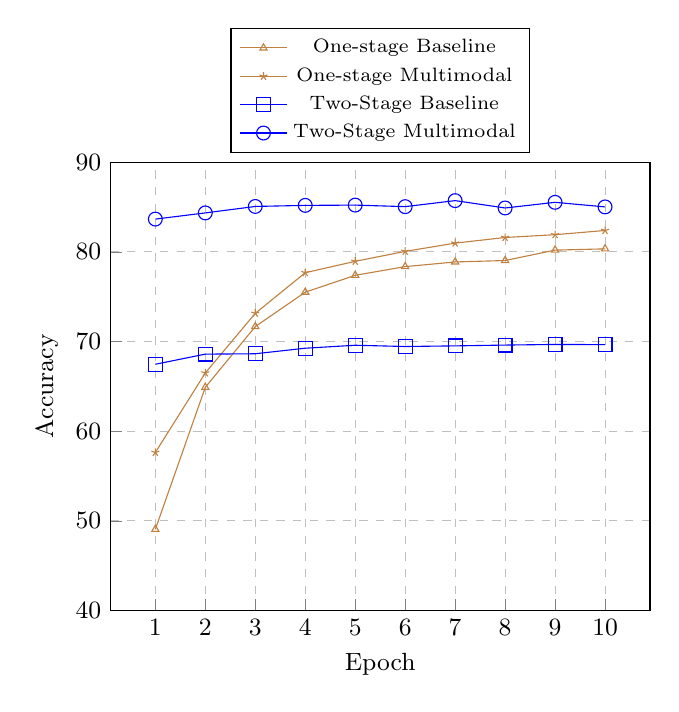
\begin{tikzpicture} \tikzset{every node}=[font=\small] 
\begin{axis} [
                align = center,
                legend style={at={(0.5,1.3)},anchor=north},
                ymin=40, ymax=90,
                xticklabels={1,2,3,4,5,6,7,8,9,10}, xtick={0,1,2,3,4,5,6,7,8,9},
                ylabel style={align=center},
                xlabel={Epoch},
                ylabel={Accuracy},
                ytick={40, 50, 60, 70, 80, 90},
                ymajorgrids=true,
                xmajorgrids=true,
                grid style=dashed,
xtick pos=bottom,
                ytick pos=left,
                ]

\addplot+[color=brown,
                    mark=triangle,
                    mark size=1.5pt,
                    ] coordinates {(0, 49.05) (1, 64.89) (2, 71.66) (3, 75.50) (4, 77.38) (5, 78.35) (6, 78.87) (7, 79.03) (8, 80.19) (9, 80.33)};\addlegendentry{\scriptsize {One-stage} Baseline}

\addplot+ [color=brown,
                    mark=star,
                    mark size=1.5pt,
                    ] coordinates { (0, 57.62)  (1, 66.49) (2, 73.14) (3, 77.67) (4, 78.94) (5, 80.05) (6, 80.97) (7, 81.60) (8, 81.91) (9, 82.38)};\addlegendentry{\scriptsize {One-stage} Multimodal}

\addplot+ [color=blue,
                    mark=square,
                    mark size=2.5pt,
                    ] coordinates { (0, 67.46)  (1, 68.59) (2, 68.63) (3, 69.25) (4, 69.58) (5, 69.44) (6, 69.51) (7, 69.60) (8, 69.67) (9, 69.65)};\addlegendentry{\scriptsize Two-Stage Baseline}

\addplot+ [color=blue,
                    mark=o,
                    mark size=2.5pt,
                    ] coordinates { (0, 83.65)  (1, 84.34) (2, 85.06) (3, 85.18) (4, 85.21) (5, 85.04) (6, 85.71) (7, 84.89) (8, 85.52) (9, 85.01)};\addlegendentry{\scriptsize Two-Stage Multimodal}

\end{axis}
\end{tikzpicture}
\vspace{-3mm}
	\caption{Accuracy curve of the {No-CoT baseline} and Multimodal-CoT variants across epochs.}\label{fig:curve}
 \vspace{-5mm}
\end{figure}

\subsection{Multimodality Boosts Convergence}
Figure \ref{fig:curve} shows the evaluation accuracy curve of the baseline and Multimodal-CoT in different training epochs. {``One-stage'' is based on the QCM$\rightarrow$A input-output format as it achieves the best performance in Table \ref{tab:pre_position} and ``Two-stage'' is our two-stage framework.} We find that the two-stage methods achieve relatively higher accuracy at the beginning than the {one-stage} baselines that generate the answer directly without CoT. However, without the vision features, the two-stage baseline could not yield better results as the training goes on due to the low-quality rationales (as observed in Section \ref{sec:prelim}). In contrast, 
using vision features helps generate more effective rationales that contribute to better answer accuracy in our two-stage multimodal variant.


\subsection{Using Different Vision Features}\label{sec:vision_features}
Different vision features may affect the model performance. We compare three widely-used types of vision features, CLIP \citep{radford2021learning}, DETR \citep{carion2020end}, and ResNet \citep{he2016deep}. CLIP and DETR are patch-like features where DETR is based on object detection. For the ResNet features, we repeat the pooled features of ResNet-50 to the same length with the text sequence to imitate the patch-like features, where each patch is the same as the pooled image features. More details of the vision features are presented in Appendix \ref{appendix:vision_features}.

\begin{table}[htb]
\vspace{-3.6mm}
    \centering\small
        \caption{Accuracy (\%) of using different vision features. \label{tab:visual_features}}
   \setlength{\tabcolsep}{10pt}
\begin{tabular}{llcc}\toprule
 {Method}  & {One-stage} & {Two-Stage}\\\midrule
\quad w/ CLIP  & 81.21 & 84.81\\
 \quad w/ DETR  & 82.57 & 84.91\\
 \quad w/ ResNet & 80.97 & 84.77\\
\bottomrule
\end{tabular}
\vspace{-3.6mm}
\end{table}

Table \ref{tab:visual_features} shows the comparative results of vision features. We observe that using vision features generally achieves better performance than the language only baseline. Specifically, DETR achieves {relatively better} performance in general. Therefore, we use DETR by default in Multimodal-CoT.

\subsection{General Effectiveness Across Backbone Models}\label{sec:backbones}
To test the generality of the benefits of our approach to other backbone models, we alter the underlying LMs to other variants in different sizes or types. As shown in Table \ref{tab:backbone}, our approach is generally effective for the widely-used backbone models.


\begin{table}[htb]
\vspace{-2mm}
    \centering\small
        \caption{Accuracy (\%) with different backbone language models. \label{tab:backbone}}
   \setlength{\tabcolsep}{2.5pt}
\begin{tabular}{llcc}\toprule
 {Method} & {Size} & {Language Only} & {Mutimodal-CoT} \\\midrule
 UnifiedQA$_\texttt{Base}$ & 223M & 80.40 & 84.91  \\
 UnifiedQA$_\texttt{Large}$ & 738M & 83.60 & 91.68\\
 \midrule
 FLAN-T5$_\texttt{Base}$ & 248M &83.42  & 85.85  \\
 FLAN-T5$_\texttt{Large}$ & 783M & 85.19& 93.02 \\
\bottomrule
\end{tabular}
\vspace{-3.6mm}
\end{table}



\subsection{Error Analysis}\label{sec:case_studies}

To better understand the behavior of Multimodal-CoT and facilitate future studies, we manually investigate randomly selected examples generated by our approach. Table \ref{tab:analysis_error} summarizes the categorization results generated by Multimodal-CoT. We randomly picked up 50 samples whose answers were correct and 50 samples whose answers were incorrect. The corresponding examples from each category are presented in Appendix \ref{appendix:case_study}.

\begin{table}[h]
    \centering\small
\vspace{-3mm}
    \caption{Categorization analysis of Multimodal-CoT.}
    \label{tab:analysis_error}
    \begin{tabular}{llc}\toprule
    Answer & CoT Category & Percentage (\%) \\
    \midrule 
    \multirow{2}{*}{Correct} &CoT is correct & 90 \\
    &CoT is incorrect & 10\\
    \midrule
    \multirow{3}{*}{Incorrect} 
    & Commonsense Mistake & 82  \\
& Logical Mistake & 12 \\
    & CoT is correct & 6 \\
    \bottomrule
\end{tabular}
\end{table}

We find that the correct samples {(i.e., whose answers are correct)} contain a certain amount of incorrect chain-of-thought (10\%). The results indicate that CoT may not always benefit the answer inference, and the model is robust to some extent --- it can predict the correct answer by ignoring incorrect rationales. For incorrect samples {(i.e., whose answers are incorrect), commonsense mistake in the CoT} is the most frequent error type (88\%). The model often makes commonsense mistakes when answering the questions requires commonsense knowledge, e.g., understand maps and counting numbers in the images (Figure \ref{fig-case-study-incorrect-fact}), and utilizing the alphabet (Figure \ref{fig-case-study-incorrect-comonsense}). The other type of mistake is a logical mistake (12\%), with contradictions in the reasoning chains  (Figure \ref{fig-case-study-incorrect-logical}). In addition, there are cases with incorrect answers while their CoT are correct (6\%) but might not be necessarily related to answer options (Figure \ref{fig-case-study-incorrect-correct}).

The analysis indicates that there are prospective directions for future studies. It is possible to improve Multimodal-CoT by (i) incorporating more informative vision features and improving language-vision interaction to be capable of understanding maps and counting numbers; (ii) injecting commonsense knowledge; (iii) applying a filtering mechanism, e.g., using only the effective CoT to infer the answer and get rid of irrelevant CoT.

\section{Conclusion}
We formally study the problem of multimodal CoT. {We propose Multimodal-CoT that incorporates language and vision modalities into a two-stage framework that separates rationale generation and answer inference, so answer inference can leverage better generated rationales from multimodal information.} With Multimodal-CoT, we show that {our method surpasses GPT-3.5 by 16 percentage points in accuracy on the ScienceQA benchmark.} Our error analysis shows that it is the potential to leverage more effective vision features, inject commonsense knowledge, and apply filtering mechanisms to improve CoT reasoning in future studies.

\bibliography{mm-cot}
\bibliographystyle{icml2023}


\newpage
\appendix
\onecolumn
\section{Extended analysis for the challenge of Multimodal-CoT}

\subsection{More Examples of Misleading by Hallucinated Rationales}\label{appendix:misleading}

According to our case studies (Section \ref{sec:misleading}), we find that the baseline tends to generate hallucinated rationales. We provide further examples as shown in Figure \ref{fig_pre_case2}.

\begin{figure*}[!htb]
  \begin{center}
   \includegraphics[width=1.0\textwidth]{figures/fig-pre-case2.pdf}
  \end{center}
  \vspace{-3mm}
  \caption{Examples of the two-stage framework without vision features (baseline) and with vision features (ours) for generating rationales and predicting answers. The upper part presents the problem details, and the lower part shows the outputs of the baseline and our method. 
  }
    \vspace{-3mm}
  \label{fig_pre_case2}
\end{figure*}



\subsection{Two-Stage Training Performance with Different Sizes of LMs.}\label{appendix:lms}

In Section \ref{sec:prelim}, we obverse that incorporating vision features helps generate more effective rationales, thus leading to improved answer accuracy. Besides incorporating vision features, it is possible to scale the LM size to mitigate the issue of incorrect rationales. Figure \ref{fig_lm_size} shows the answer accuracy with UnifiedQA$_\texttt{Base}$ and UnifiedQA$_\texttt{Large}$. When using a larger LM, the accuracy of the baseline (w/o vision features) is boosted. The result indicates that scaling the LM is possible to mitigate the issue of incorrect rationales. However, the performance is still much inferior to using vision features. The result further verifies the effectiveness of our Multimodal-CoT with different sizes of LMs.




\begin{figure}[htb]
  \begin{center}
{
\pgfplotsset{compat=1.13,
    /pgfplots/ybar legend/.style={
    /pgfplots/legend image code/.code={\draw[##1,/tikz/.cd,yshift=-0.25em]
        (0cm,0cm) rectangle (7pt,0.8em);},
   },
}
\pgfplotsset{width=7.0cm, height=5.5cm}
    \centering


    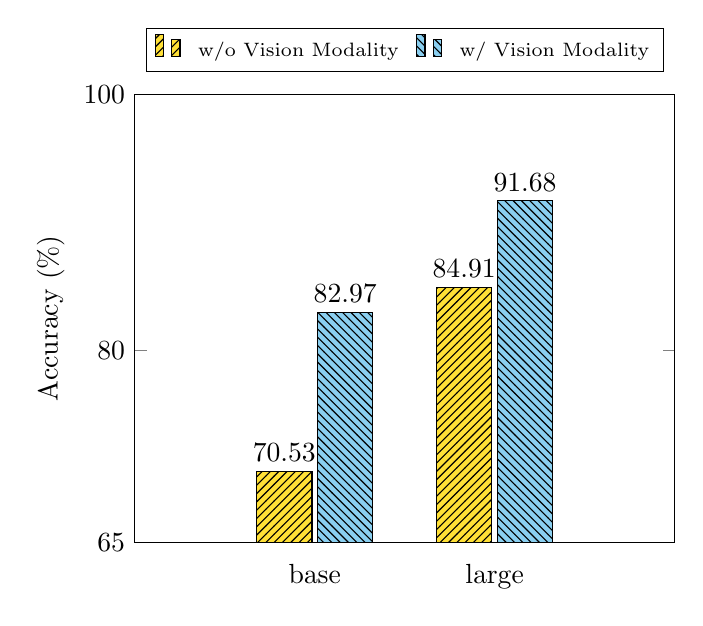
\begin{tikzpicture}  
        \begin{axis}  
        [  
            ybar,
            ymin=65, ymax=100,
            ytick={65,80,100},
            major x tick style = transparent,
            bar width=20pt,
            enlarge x limits=1.0,
            ylabel={Accuracy (\%)},
            symbolic x coords={0,1},  
            xtick=data,  
            xticklabels={base, large},
            nodes near coords,  
            nodes near coords align={vertical},  
        legend cell align=left,
         legend columns=2 row=1,
                legend style={
                        at={(0.5,1.05)},
                        anchor=south,
                        column sep=1ex,
                        font=\scriptsize,
                }
            ]  
        \addplot[ybar, fill=bananayellow,  postaction={pattern=north east lines}] coordinates {
            (0,70.53)(1, 84.91)
        };  
        \addplot[ybar, fill=babyblue,  postaction={pattern=north west lines}] coordinates {
            (0, 82.97)(1, 91.68)
        };
        \legend{w/o Vision Modality, w/ Vision Modality} 
        \end{axis}  
    \end{tikzpicture}
\caption{
   Answer accuracy with different sizes of LMs.\label{fig_lm_size}
    }
}
  \end{center}
  \label{fig_scaling}
\end{figure} 
\section{Experimental Details}

\subsection{Baseline Methods}\label{app-sec:baseline}
Following \citet{lu2022learn}, our baselines include three types of methods: 

(i) Visual question answering (VQA) models \citep{yu2019mcan,Anderson2017up,Kim2018,gao2019dynamic,lu2021iconqa,li2019visualbert}. The VQA baselines take the question, the context, and choices as the textual input, take the image as the vision input, and predict the score distribution over choice
candidates via a linear classifier.

(ii) Text-to-text LM models. UnifiedQA \citep{khashabi2020unifiedqa} is adopted as it is the best fine-tuning model in \citet{lu2022learn}. UnifiedQA takes the textual information as the input and outputs the answer option. The image is converted into a caption extracted by an image captioning
model based on ViT and GPT-2.\footnote{\url{https://huggingface.co/nlpconnect/vit-gpt2-image-captioning}.} UnifiedQA treats our task as a text generation problem. In \citet{lu2022learn}, it is trained to generate a target answer text, i.e., one of the candidate options. Then, the most similar option is selected
as the final prediction to evaluate the question answering accuracy.

(iii) GPT-3.5 models \citep{chen2020big} based on the text-davinci-002 engine. The inference is based on the few-shot prompting, where two in-context examples from the training set are concatenated before the test instance.

For UnifiedQA and GPT-3.5, CoT is applied after the answer \citep{lu2022learn}. Besides the above baselines, we develop a stronger baseline with a slight modification of the output format of UnifiedQA. Instead of predicting the answer texts, our baseline directly predicts the choice, e.g., \textit{the answer is B}. This setting helps our baseline achieve better results than the existing UnifiedQA. Therefore, we use the stronger method as the language only baseline for analysis. 

\subsection{Details of Vision Features}\label{appendix:vision_features}
In Section \ref{sec:vision_features}, we compared four types of vision features, CLIP \citep{radford2021learning}, DETR \citep{carion2020end}, and ResNet \citep{he2016deep}. The specific models are: (i) CLIP: RN101;\footnote{\url{https://github.com/jianjieluo/OpenAI-CLIP-Feature}.} (ii) DETR: \textit{detr\_resnet101\_dc5};\footnote{\url{https://github.com/facebookresearch/detr}.} (iii) ResNet: we use the averaged pooled features of a pre-trained ResNet50 CNN. Table \ref{tab:visual_dimension} presents the dimension of the vision features (after the function \textrm{VisionExtractor}($\cdot$) in Eq. \ref{eq:extractor}). For ResNet-50, we repeat the 
pooled features of ResNet-50 to the same length as the text sequence to imitate the patch-like features, where each patch is the same as the pooled image features. 

\begin{table}[htb]
\centering\small
        \caption{Dimension of vision features\label{tab:visual_dimension}}
\begin{tabular}{llcc}\toprule
 {Method} & {Dimension} \\\midrule
 \quad  CLIP & (49, 2048) \\
 \quad  DETR& (100, 256) \\
 \quad  ResNet & (512, 2048) \\
\bottomrule
\end{tabular}
\end{table}

\section{Examples of Case Studies}\label{appendix:case_study}
To better understand the behavior of Multimodal-CoT, we manually investigate randomly selected examples generated by our approach. Table \ref{tab:analysis_error} summarizes the categorization results generated by Multimodal-CoT. We randomly picked up 50 samples whose prediction results were correct and 50 samples whose prediction results were incorrect.

We find that the correct samples contain a certain amount of incorrect chain-of-thought.
As shown in Figure \ref{fig-case-study-correct-ans}(b), the model generates the incorrect rationale, ``\textit{Animals cannot their food by digesting other organisms}" but the predicted answer is correct. The result indicates that CoT may not always benefit the answer inference, and the model is robust to some extent --- it can predict the correct answer by ignoring incorrect rationales.

\begin{figure*}[htb]
  \begin{center}
   \includegraphics[width=1\textwidth]{figures/fig-case-study-correct-ans.pdf}
  \end{center}
\caption{Examples of answers are correct while the CoT is correct (a) or incorrect (b).}
\label{fig-case-study-correct-ans}
\end{figure*}

For incorrect samples, commonsense mistake is the most frequent error type. The model also makes commonsense mistakes when answering the questions requires commonsense knowledge, e.g., understand maps and counting numbers in the images (Figure \ref{fig-case-study-incorrect-fact}), and utilizing the alphabet (Figure \ref{fig-case-study-incorrect-comonsense}). The other type of mistake is the logical mistake, where there are contradictions in the reasoning chains (Figure \ref{fig-case-study-incorrect-logical}). In addition, there are cases that the CoT is correct but might not be necessarily related to answer options; thus the model chooses the incorrect answer.

\begin{figure*}[htb]
  \begin{center}
   \includegraphics[width=1\textwidth]{figures/fig-case-study-incorrect-fact.pdf}
  \end{center}
\caption{Examples of commonsense mistakes about understanding maps and counting numbers.}
\label{fig-case-study-incorrect-fact}
\end{figure*}

\begin{figure*}[htb]
  \begin{center}
   \includegraphics[width=1\textwidth]{figures/fig-case-study-incorrect-comonsense.pdf}
  \end{center}
\caption{Examples of commonsense mistakes about utilizing alphabet.}
\label{fig-case-study-incorrect-comonsense}
\end{figure*}

\begin{figure*}[htb]
  \begin{center}
   \includegraphics[width=1\textwidth]{figures/fig-case-study-incorrect-logical.pdf}
  \end{center}
\caption{Examples of logical mistakes.}
\label{fig-case-study-incorrect-logical}
\end{figure*}

\begin{figure*}[htb]
  \begin{center}
   \includegraphics[width=1\textwidth]{figures/fig-case-study-incorrect-correct.pdf}
  \end{center}
\caption{Examples of answers are incorrect while the CoT is correct.}
\label{fig-case-study-incorrect-correct}
\end{figure*}

The analysis indicates that there are prospective directions for future studies. On the one hand, it is possible to improve the quality of CoT by (i) using more fine-grained interaction of language and vision features; and (ii) injecting commonsense knowledge. On the other hand, applying a filtering mechanism to using only the effective CoT to infer the answer and eliminate irrelevant CoT.



\end{document}
